%%% LaTeX Template
%%% This template can be used for both articles and reports.
%%%
%%% Copyright: http://www.howtotex.com/
%%% Date: February 2011

%%% Preamble
\documentclass[paper=a4, fontsize=11pt]{scrartcl}	% Article class of KOMA-script with 11pt font and a4 format
\usepackage[margin=0.7in]{geometry}
\usepackage[english]{babel}															% English language/hyphenation
\usepackage[protrusion=true,expansion=true]{microtype}				% Better typography
\usepackage{amsmath,amsfonts,amsthm}										% Math packages
%\usepackage{color,transparent}													% If you use color and/or transparency
\usepackage[hang, small,labelfont=bf,up,textfont=it,up]{caption}	% Custom captions under/above floats
\usepackage{epstopdf}																	% Converts .eps to .pdf
\usepackage{subfig}																		% Subfigures
\usepackage{booktabs}																	% Nicer tables
\usepackage[pdftex]{graphicx}
\usepackage{listings}

%%% Advanced verbatim environment
\usepackage{verbatim}
\usepackage{fancyvrb}
\DefineShortVerb{\|}								% delimiter to display inline verbatim text


%%% Custom sectioning (sectsty package)
\usepackage{sectsty}								% Custom sectioning (see below)
\allsectionsfont{%									% Change font of al section commands
	\usefont{OT1}{bch}{b}{n}%					% bch-b-n: CharterBT-Bold font
%	\hspace{15pt}%									% Uncomment for indentation
	}

\sectionfont{%										% Change font of \section command
	\usefont{OT1}{bch}{b}{n}%					% bch-b-n: CharterBT-Bold font
	\sectionrule{0pt}{0pt}{-5pt}{0.8pt}%	% Horizontal rule below section
	}


%%% Custom headers/footers (fancyhdr package)
\usepackage{fancyhdr}
\pagestyle{fancyplain}
\fancyhead{}														% No page header
\fancyfoot[C]{\thepage}										% Pagenumbering at center of footer
\renewcommand{\headrulewidth}{0pt}				% Remove header underlines
\renewcommand{\footrulewidth}{0pt}				% Remove footer underlines
\setlength{\headheight}{13.6pt}

%%% Equation and float numbering
\numberwithin{equation}{section}															% Equationnumbering: section.eq#
\numberwithin{figure}{section}																% Figurenumbering: section.fig#
\numberwithin{table}{section}

\usepackage[parfill]{parskip}
\usepackage{float}
\usepackage{hyperref}
\usepackage[numbers]{natbib}															% Tablenumbering: section.tab#


%%% Title
\title{
	\vspace{-0.5in} 	\usefont{OT1}{bch}{b}{n}
        SEM2220: Mobile Web Assignment \
}

% Authors
\author{
	\usefont{OT1}{bch}{m}{n} Samuel Jackson
	\\ \usefont{OT1}{bch}{m}{n} University Of Aberystwyth
	\\   \texttt{slj11@aber.ac.uk}
}

\date{\today}

\begin{document}

\maketitle

\clearpage

\section{Introduction}
\label{sec:introduction}
This report provides the documentation for the mobile web assignment for SEM2220. The aim of this assignment is to add some additional functionality to an existing code base comprising of a responsive website wrapped as a PhoneGap application for deployment as a native mobile application. Section \ref{sec:dynamic-lists} discusses the implementation of a dynamic sessions lists as specified in the assignment brief. This section will discuss both the final solution and any problems encountered. Section \ref{sec:dynamic-maps} discusses an additional feature implemented for ``flair'' marks. Again this will focus on the solution produced and outline any difficulties encountered along the way.

Before beginning to implement either of these two parts I first took the existing code base and converted it into a PhoneGap application, following the steps outlined during the practical workshops. I also wrote a small script that builds locally and deploys the project to an Android device connected via USB. This enabled me to rapidly deploy the application to a real device for testing in both of the following sections. The full PhoneGap project, including the deployment script and the source for this document are supplied in the zip folder submission.

\section{Implementing the Dynamic Sessions List}
\label{sec:dynamic-lists}
Implementing the dynamic sessions list involved interpreting the existing code base and then implementing several steps to produce a working sessions list. The existing code base already implemented the basic functionality of the website, including navigation between pages and setting up a local database with test data. 

There were two main areas that needed to be extended in order to get dynamic sessions loading working proper which were marked with inline comments. The first of these was in the \textit{Controller.js} file in a function called \textit{renderSessionsList}. This function acts as an event handler which responds to sessions being loaded from the local database. It's purpose is to render the data received from the database query as HTML code. This function should be concerned with how sessions are presented to the user.

The second place that required changes in order for the code to work was in the \textit{DataContext.js} file. This file is responsible for controlling operations on the local database. All that was required in this file was to implement the function \textit{querySessions} to retrieve session data from the database.

The code in the \textit{DataContext.js} file is possibly the simplest code modification. It executes an SQL select statement to pull the session data from the table in the local database for the first day (as indicated by the comments). The response is then passed to a handler function called \textit{handleSessionsLoaded}. This performs two duties. Firstly it converts the loaded \textit{SQLResultSet} to a vanilla Javascript array. I chose to do this so that the presentation code in \textit{Controller.js} could use generic array manipulation functions (e.g. \textit{map, forEach, reduce}) which are not present on the result object. This also hides the format of the underlying data storage system resulting in better decoupling. Its second duty is to call the \textit{processorFunc} with the query result (now as an array). This \textit{processorFunc} is set to the event handler \textit{renderSessionsList}, yielding control back to the \textit{Controller.js}.

The \textit{processorFunc} in the \textit{Controller.js} file converts the returned array of session data into HTML elements which match the format of the original static structure of the sessions list provided in the module tutorials. The resulting HTML elements are then inserted into the DOM using the jQuery library. Once the new HTML content has been inserted into the DOM jQuery Mobile (JQM) event handlers must be bound to the new content. According to the JQM documentation \cite{jqm-scripting-docs} newly created components need to be initialised by calling \textit{.trigger(`create')} on the parent HTML element of the newly inserted HTML.

Finally, a new filterable widget is added to the content of the page. This is created after the listview widget has been initialised so that the events and styling of the filter widget are setup correctly. One of the issues I encountered when implementing this part of the project was that widgets which were not created or setup correctly caused either the functionality to break or weird CSS styling (specifically extra padding above the filter to appear).


\section{Implementing Interactive Venue Maps}
\label{sec:dynamic-maps}
For the additional ``flair'' marks for this assignment I chose to implement interactive google maps in the project. This feature loads the venues for the current day from the local database and shows them as markers on the map. Clicking/tapping on the marker will cause an info window to appear with the name of the location shown.

There are several parts to this feature. Firstly, instead of generating a static map from the Google maps API I imported the full JavaScript library inside the \textit{index.html} file. This provides a much richer API for creating maps which are both more pleasant for the user and interactive, resulting in a much richer UI experience.

\begin{figure}[H]
\centering
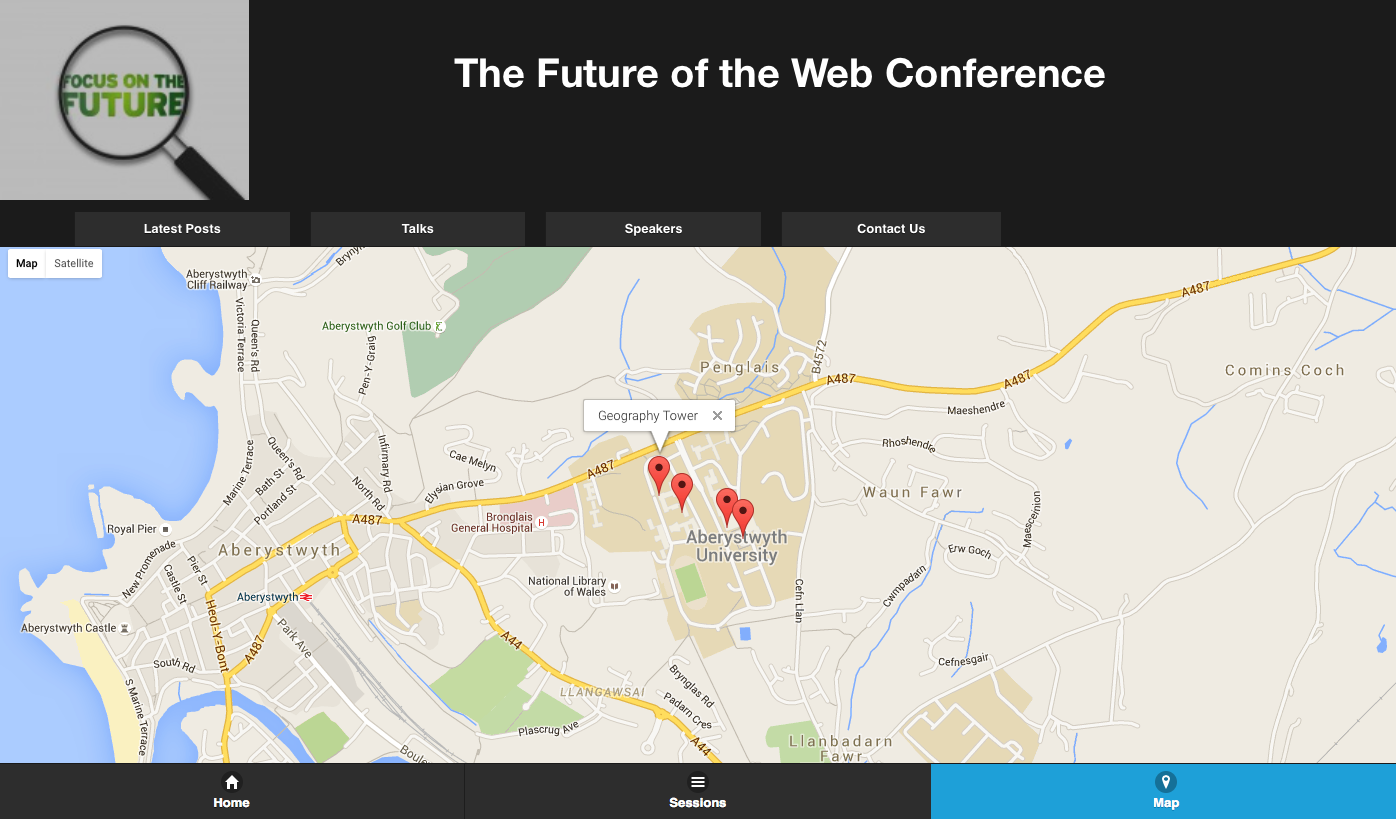
\includegraphics[width=0.9\textwidth]{google-maps.png}
\caption{Screen capture showing the maps page with markers for the venues and an info window showing the location name}
\label{fig:google-maps}
\end{figure}

The next part of this feature required me to load the venues from the local database when the user clicks on the map page so that they can be displayed as markers. To do this I followed a methodology very similar to how I implemented the first part of this assignment. Specifically I added an additional function called \textit{queryLocations} to the \textit{DataContext.js} file. This selects all of the venues currently present in the database and converts the result set to an array before calling the \textit{processorFunc}. This time the \textit{processorFunc} is set to a different handler that iterates over the returned data and creates markers using the Google API in \textit{Controller.js}.

Several additional changes were made to the existing map code in the \textit{Controller.js}. The \textit{handle\_geolocation\_query} was function has been changed to remove the static map creation and instead:

\begin{itemize}
	\item Sets up a new Google Map in the content area of the page
	\item Requests to load venue data from the local database
	\item Converts each venue to an interactive map marker
\end{itemize}

I found that this got Google maps working but encountered several additional issues which needed to be addressed. Firstly, when resizing the browser window the centre location of the map would not adjust itself accordingly. This meant that the location that the map was centred over would not adjust itself to keep the middle section always visible. I found that this was easily fixed by creating an event handler for the resize event handler available in the Google maps API (via the stack overflow question \cite{google-maps-stackoverflow}).

The second issue I found after implementing this feature was that the maps would not work on a mobile device, but worked fine in a normal web browser. This is a good example of where Google Chrome's remote debugging tools came in handy during this assignment.

\begin{figure}[H]
\centering
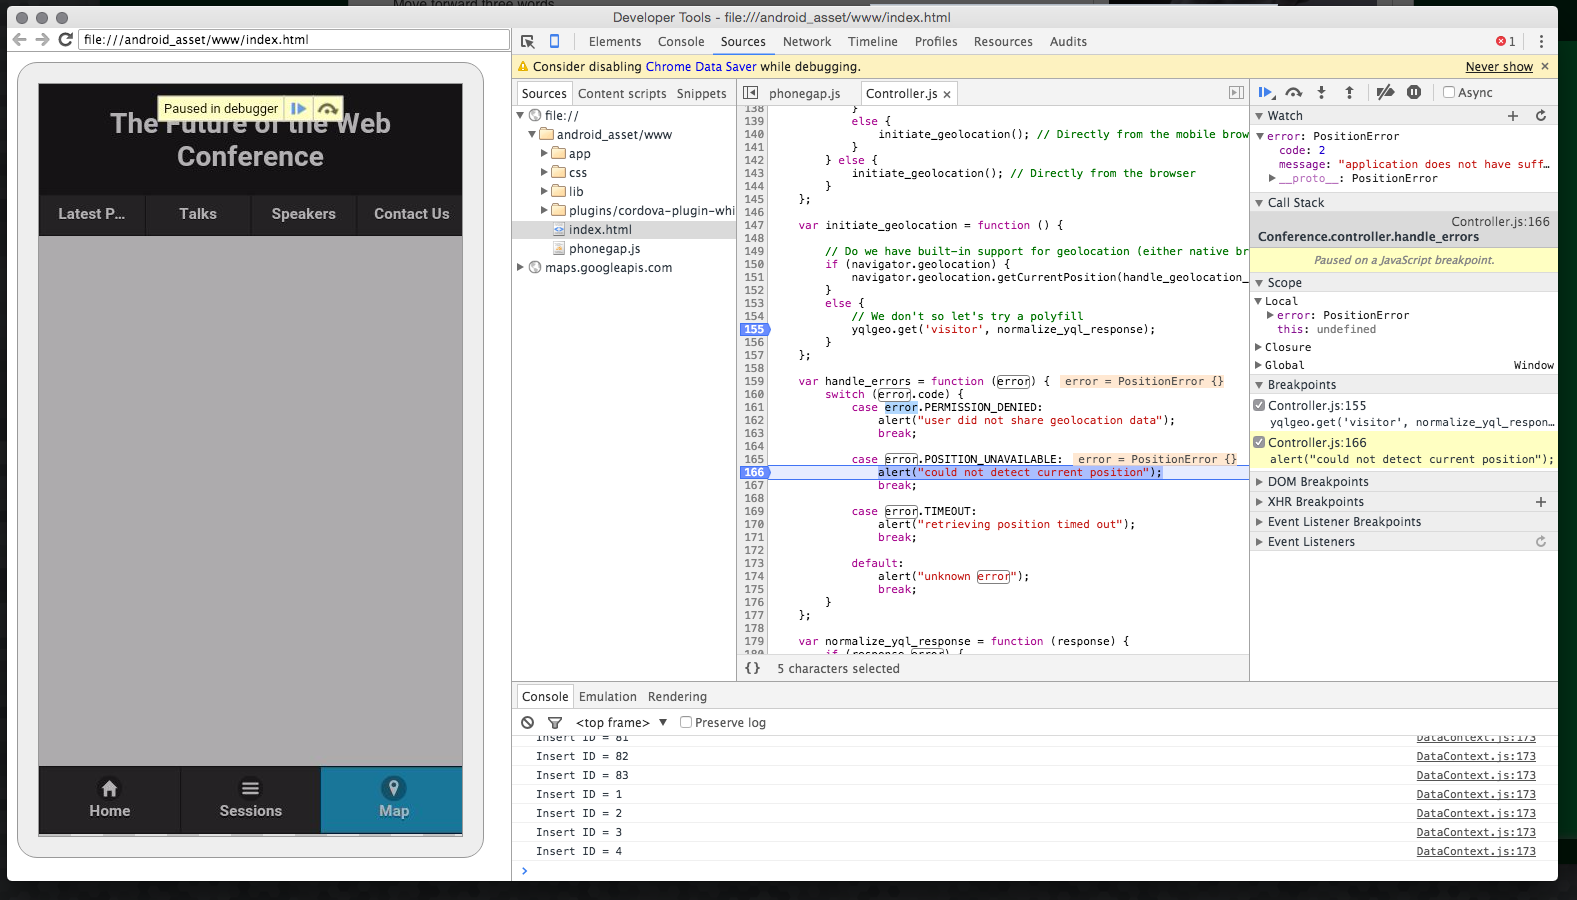
\includegraphics[width=0.9\textwidth]{mobile-debugging.png}
\caption{Screen capture showing Chrome's remote debugging tools inspecting code running on my Android phone. This shows me examining the the error variable I was receiving which stated my application had insufficient user permissions. This version used Chrome Canary so that the WebView could be debugged directly.}
\label{fig:google-maps}
\end{figure}

Using the remote debugger tool I was able to track down the error to the fact that the application had insufficient user permissions enabled to detect the users current location. I was able to easily fix this problem once I understood it by adding the following user permission to android manifest file:

\begin{lstlisting}
<uses-permission android:name=``android.permission.ACCESS_FINE_LOCATION'' />	
\end{lstlisting}

\section{Discussion}
\label{sec:discussion}
This implementation is obviously limited by the fact that the sessions list only returns data for the first day. The first major improvement would be to actually get this working correctly with the database for multiple days rather than being hard coded into the SQL query. 

Another improvement would be to swap from the current implementation which uses the Google maps JavaScript API to use the Cordova  plugin. This would bring native maps support to the project which could bring a performance improvement. However this plugin has issues with the PhoneGap/Cordova version used in this assignment so I chose to only use the JavaScript API. Upgrading to use the plugin in future work should not be a huge issue based on the current implementation.

One thing which I found noticed with this assignment was the difficulty in testing the application. Testing that the application works correctly is easy in a web context, but testing to be certain that the application works correctly is difficult when you are targeting so many devices, although the Chrome debug tools go a long way to helping. Automated unit tests for the website would not necessarily guarantee the successful deployment to a device (as in the debugging example in the previous section). I think this remains an open challenge for hybrid apps.

\section{Self Evaluation}
Overall I would give this assignment a 70\%. I feel this grade is justified for the following reasons: I have implemented all of the requirements of the assignment brief and I feel I have clearly documented the changes made in this document and my experiences with testing/debugging the application. I also feel that while I am far from a JavaScript expert I have written code that is reasonably clean and well commented. I feel that the implementation of interactive Google maps should gain me some additional flair marks, but obviously more work could be done to the enhance the application such as the additional suggestions on the brief. Taking all of these points together I feel that a grade of 70\% is not an unreasonable expectation.


\clearpage
\bibliographystyle{unsrtnat}
\bibliography{references}
\end{document}
